\documentclass{ieeeaccess}
\usepackage{cite}
\usepackage{amsmath,amssymb,amsfonts}
\usepackage{algorithmic}
\usepackage{graphicx}
\usepackage{textcomp}
\usepackage{booktabs}
\usepackage{multirow}
\usepackage{hyperref}

% ORCID icon command - links to ORCID profile
\newcommand{\orcidicon}[1]{\href{https://orcid.org/#1}{\textcolor{blue}{ORCID}}}

\def\BibTeX{{\rm B\kern-.05em{\sc i\kern-.025em b}\kern-.08em
    T\kern-.1667em\lower.7ex\hbox{E}\kern-.125emX}}

\begin{document}
\history{Date of publication xxxx 00, 0000, date of current version xxxx 00, 0000.}
\doi{10.1109/ACCESS.2026.XXXXXXX}

\title{KAN-inspired Universal Relaxation Network for Automatic Discovery of Physical Relaxation Mechanisms with Direct Circuit Synthesis}

\author{
\uppercase{Kengo Sugahara}\authorrefmark{1},\orcidicon{0000-0002-2200-311X} and
\uppercase{Yuki Sato}\authorrefmark{2},\orcidicon{0000-0002-4052-5966}
}

\address[1]{Faculty of Science and Engineering, Kindai University, Higashi-Osaka 577-8502, Japan}
\address[2]{Department of Electrical and Electronic Engineering, Aoyama Gakuin University, Sagamihara 252-5258, Japan}

\tfootnote{This work was supported in part by JSPS KAKENHI.}

\markboth
{Sugahara and Y. Sato: KAN-inspired Universal Relaxation Network}
{Sugahara and Y. Sato: KAN-inspired Universal Relaxation Network}

\corresp{Corresponding author: Kengo Sugahara (e-mail: sugahara@kindai.ac.jp).}

\begin{abstract}
We propose the Universal Relaxation Network (URN), a KAN-inspired approach for automatic discovery of physical relaxation mechanisms from frequency-domain impedance data. Unlike Vector Fitting (VF), which uses pole-residue representations that can produce unstable models, URN employs 29 circuit-compatible basis functions derived from established physical models (Debye, Cole-Cole, Warburg, skin effect). A learnable frequency-dependent attention mechanism $\alpha_k(\omega) = \text{softmax}(\text{MLP}(\log\omega))$ automatically emphasizes relevant basis functions at different frequency ranges. Through L1-regularized sparse optimization, URN automatically selects dominant mechanisms and directly synthesizes SPICE-compatible RLC ladder networks. The pole-free formulation guarantees structural stability while providing physically interpretable parameters. \textbf{Ablation study on real-world data} demonstrates that attention improves accuracy by 79--83\% compared to uniform weighting. Cross-domain validation using TDK MnZn ferrite datasheet measurements and NASA Li-ion battery EIS data achieves 1.1--21.9\% fitting error. Time-domain SPICE simulations verify absence of spurious ringing. Open-source PyTorch implementation with benchmark datasets is available for reproducibility.
\end{abstract}

\begin{keywords}
Circuit synthesis, Cole-Cole relaxation, electrochemical impedance spectroscopy, impedance modeling, Kolmogorov-Arnold networks, SPICE simulation, Vector Fitting, Warburg impedance.
\end{keywords}

\titlepgskip=-15pt

\maketitle

%===============================================================================
\section{Introduction}
\label{sec:introduction}
%===============================================================================

\subsection{Time-Domain Analysis in Power Electronics}

Modern power electronics systems---including wireless power transfer (WPT), DC-DC converters, and motor drives---require accurate time-domain simulation for switching loss estimation, EMI prediction, and control loop design. Circuit simulators such as SPICE \cite{nagel1975spice2} and their derivatives (LTspice, PSIM, PLECS) form the backbone of power electronics design workflows.

A critical challenge is modeling frequency-dependent components: magnetic cores with complex permeability \cite{snelling1988soft}, winding conductors with skin and proximity effects \cite{dowell1966eddy,hurley2000optimizing}, and electrochemical cells with diffusion dynamics \cite{barsoukov2018impedance}. These components exhibit impedance that varies over multiple decades of frequency, directly affecting:
\begin{itemize}
\item \textbf{Switching transients}: Core and winding losses depend on harmonic content
\item \textbf{EMI filtering}: High-frequency impedance determines filter effectiveness
\item \textbf{Control stability}: Frequency-dependent phase shifts affect loop gain margins
\item \textbf{Thermal design}: Accurate loss estimation prevents overheating
\end{itemize}

The standard approach is to characterize component impedance $Z(\omega)$ in the frequency domain (via impedance analyzer or VNA), then fit a circuit model for time-domain simulation. The quality of this fitting directly determines simulation accuracy.

\subsection{Vector Fitting: Industry Standard with Known Limitations}

Vector Fitting (VF) \cite{gustavsen1999rational,gustavsen2006improving} is the \textit{de facto} industry standard for rational approximation of frequency responses, embedded in commercial tools (Keysight ADS, CST, Cadence) and widely trusted by power electronics engineers. VF represents impedance as:
\begin{equation}
Z(s) = \sum_{n=1}^{N} \frac{c_n}{s - a_n} + d + se
\label{eq:vf}
\end{equation}
where $a_n$ are poles and $c_n$ are residues. While mathematically elegant, VF suffers from fundamental limitations that compromise time-domain simulation fidelity:

\begin{enumerate}
\item \textbf{Pole initialization sensitivity}: VF performance depends critically on initial pole placement. Conservative initialization (damping ratio $\zeta \approx 0.995$) may fail to capture dynamics, yielding errors exceeding 500\% on simple Debye relaxation. Aggressive initialization ($\zeta \approx 0.1$) produces weakly-damped poles that cause \textit{spurious ringing} in time-domain simulations---oscillations that do not exist in the physical system.

\item \textbf{Time-domain instability}: Weakly-damped poles with natural frequencies between measurement points can produce unbounded oscillations in transient simulation. Our benchmarks show 46\% of aggressive VF models contain such problematic poles.

\item \textbf{Lack of physical interpretability}: Poles and residues have no correspondence to physical mechanisms. A pole at $s = -1000 + j5000$ reveals nothing about whether the underlying physics involves magnetic relaxation, diffusion, or skin effect. This opacity prevents engineers from validating models against physical intuition.

\item \textbf{Model order selection}: Users must specify pole count \textit{a priori}. Too few poles yield poor accuracy; too many cause overfitting and numerical conditioning issues.

\item \textbf{Circuit synthesis complexity}: Converting pole-residue models to SPICE netlists requires Foster or Cauer synthesis \cite{foster1924reactance,cauer1958synthesis}, which may produce negative component values requiring workarounds (controlled sources, negative resistors).
\end{enumerate}

\subsection{KAN: A New Paradigm for Function Approximation}

The recently proposed Kolmogorov-Arnold Networks (KAN) \cite{liu2024kan} offer a fundamentally different approach to function approximation. Based on the Kolmogorov-Arnold representation theorem \cite{kolmogorov1957representation,arnold1957functions}:
\begin{equation}
f(x_1, \ldots, x_n) = \sum_{q=0}^{2n} \Phi_q \left( \sum_{p=1}^{n} \phi_{q,p}(x_p) \right)
\end{equation}
KAN replaces fixed activation functions in neural networks with \textit{learnable univariate functions} on network edges, typically implemented as B-splines.

KAN's key innovations include:
\begin{itemize}
\item \textbf{Interpretability}: Learned functions can be inspected and symbolically simplified
\item \textbf{Accuracy}: Outperforms MLPs on scientific computing tasks
\item \textbf{Efficiency}: Smaller networks achieve comparable accuracy
\end{itemize}

However, directly applying KAN to impedance modeling faces challenges:
\begin{itemize}
\item Spline-based functions do not map to physical circuits
\item No guarantee of passivity or stability
\item SPICE netlist generation is non-trivial
\end{itemize}

\subsection{URN: KAN Philosophy with Circuit Constraints}

We propose the Universal Relaxation Network (URN), which adapts KAN's philosophy of \textit{learnable basis functions} while constraining the search space to \textit{circuit-synthesizable} forms. For impedance modeling, the representation becomes:
\begin{equation}
Z(\omega) = Z_\infty + \sum_{i=1}^{M} w_i \cdot \phi_i(\omega; \theta_i)
\label{eq:urn}
\end{equation}
where $\phi_i$ are \textit{physically-motivated basis functions} (Debye, Cole-Cole, Warburg, skin effect, etc.), $\theta_i$ are physical parameters (relaxation time $\tau$, exponent $\alpha$), and $w_i$ are sparse weights selected by L1 regularization.

Table~\ref{tab:physical_mechanisms} summarizes the basis functions and their power electronics applications.

\begin{table}[!t]
\caption{Physical Relaxation Mechanisms in Power Electronics}
\label{tab:physical_mechanisms}
\centering
\begin{tabular}{@{}lll@{}}
\toprule
\textbf{Mechanism} & \textbf{Impedance Form} & \textbf{Application} \\
\midrule
Debye & $\frac{1}{1+j\omega\tau}$ & Ferrite permeability \\
Cole-Cole & $\frac{1}{1+(j\omega\tau)^\alpha}$ & Non-ideal magnetics \\
Warburg & $\frac{1}{\sqrt{j\omega}}$ & Battery diffusion \\
Skin effect & $\xi \coth(\xi)$ & Winding AC resistance \\
CPE & $(j\omega)^{-n}$ & Electrode interfaces \\
\bottomrule
\end{tabular}
\end{table}

The key insight is that while KAN discovers arbitrary functions via splines, URN discovers \textit{which physical mechanisms} are present. This trades generality for:
\begin{itemize}
\item \textbf{Direct SPICE synthesis}: Each basis maps to an RLC ladder
\item \textbf{Physical interpretability}: $\tau$, $\alpha$, $n$ have measurable meanings
\item \textbf{Guaranteed stability}: All bases derive from passive systems
\item \textbf{Time-domain fidelity}: No spurious ringing from artificial poles
\end{itemize}

\textbf{Positioning}: URN is not a replacement for VF in all applications. VF excels for broadband S-parameter fitting where physical interpretation is unnecessary. URN targets applications where (1) physical mechanism identification aids validation, (2) time-domain stability is critical, and (3) the underlying physics involves known relaxation mechanisms (ferrites, batteries, skin effect).

\subsection{Contributions}

This paper presents URN with the following contributions:

\begin{enumerate}
\item \textbf{Physics-informed basis library}: 29 circuit-compatible functions covering relaxation (Debye, Cole-Cole, Havriliak-Negami), diffusion (Warburg, Gerischer), and distributed effects (CPE, skin effect).

\item \textbf{Frequency-dependent attention}: Learnable MLP-based attention $\alpha_k(\omega) = \text{softmax}(\text{MLP}(\log\omega))$ automatically emphasizes relevant basis functions at different frequency ranges. Ablation study on real data demonstrates 79--83\% accuracy improvement.

\item \textbf{Automatic mechanism discovery}: L1-regularized sparse optimization selects dominant mechanisms without manual model order specification.

\item \textbf{Guaranteed circuit compatibility}: Each basis maps to RLC ladders via Valsa \cite{valsa2013rc}, Charef \cite{charef1992fractal}, and Dowell \cite{dowell1966eddy} methods with automatic stage determination.

\item \textbf{Pole-free formulation}: Eliminates spurious resonances that plague VF in time-domain simulation.

\item \textbf{Real-world validation}: Cross-domain validation using TDK MnZn ferrite datasheet measurements (PC47, PC50, PC95, PC200) and NASA 18650 Li-ion battery EIS data achieves 1.1--21.9\% fitting error across diverse applications.
\end{enumerate}

\subsection{Paper Organization}

Section~\ref{sec:basis} describes the KAN-inspired insight and circuit-compatible basis library. Section~\ref{sec:method} presents the training algorithm. Section~\ref{sec:kan_features} details five advanced KAN-inspired features: adaptive grid refinement, hierarchical decomposition, attention-based selection, learnable exponents, and symbolic discovery. Section~\ref{sec:results} provides benchmark results with emphasis on the pole-free advantage, experimental validation with real-world data, and time-domain simulation verification. Section~\ref{sec:theory} addresses theoretical considerations including convergence analysis, hyperparameter sensitivity, computational cost comparison, and clarification of the ``KAN-ness'' terminology. Section~\ref{sec:discussion} identifies target applications. Section~\ref{sec:conclusion} concludes.

%===============================================================================
\section{Circuit-Compatible Basis Library}
\label{sec:basis}
%===============================================================================

\subsection{The KAN-Inspired Insight}

The central insight behind URN stems from a critical observation about KAN \cite{liu2024kan} and its relationship to function approximation in physical systems.

KAN's key innovation is replacing fixed activation functions (ReLU, sigmoid) with \textit{learnable univariate functions}---typically B-splines---on network edges. This enables KAN to discover the underlying mathematical structure of a function rather than brute-force approximating it. For scientific computing, this yields significant advantages: smaller networks, better accuracy, and \textit{symbolic interpretability}.

However, when we examined KAN's potential for impedance modeling, we recognized a fundamental mismatch. While KAN discovers arbitrary univariate functions, SPICE simulation requires \textit{circuit-compatible} functions---impedances that can be realized as RLC networks. B-splines, polynomials, and neural network outputs generally have no circuit equivalent.

This led to our key insight: \textit{What if we could use KAN's philosophy of learnable basis functions, but constrain the search space to physically-meaningful, circuit-synthesizable forms?}

The answer is URN's basis library. Instead of learning arbitrary spline knots, we learn:
\begin{enumerate}
\item \textbf{Which physical mechanisms} are active (Debye, Cole-Cole, Warburg, skin effect, etc.)
\item \textbf{Their physical parameters} (relaxation time $\tau$, exponent $\alpha$, etc.)
\item \textbf{Their relative contributions} (sparse weights $w_i$)
\end{enumerate}

This constraint is not a limitation---it is the source of URN's power. Table~\ref{tab:kan_comparison} summarizes the key differences between standard KAN and URN.

\begin{table}[!t]
\caption{Comparison: Standard KAN vs URN}
\label{tab:kan_comparison}
\centering
\begin{tabular}{@{}lll@{}}
\toprule
\textbf{Aspect} & \textbf{Standard KAN} & \textbf{URN} \\
\midrule
Basis functions & B-splines (arbitrary) & Physical models \\
Learnable params & Spline knots & $\tau$, $\alpha$, weights \\
Output space & Any function & Circuit-realizable \\
Interpretability & Symbolic simplification & Physical mechanisms \\
Passivity & Not guaranteed & By construction \\
SPICE synthesis & Not possible & Direct mapping \\
\bottomrule
\end{tabular}
\end{table}

By restricting to circuit-compatible bases, we guarantee:
\begin{itemize}
\item Every output can be synthesized as an RLC ladder
\item All learned parameters have physical units and meanings
\item Passivity and stability are structural properties, not post-hoc corrections
\item Time-domain simulation is free of spurious oscillations
\end{itemize}

\subsection{Basis Function Categories}

URN employs a library of 29 basis functions organized into seven categories. Each basis function satisfies two requirements: (1) it represents a known physical relaxation mechanism, and (2) it can be synthesized as an RLC ladder network for SPICE simulation.

\subsection{Relaxation Functions}

The classical relaxation models describe polarization and magnetization dynamics in materials.

\subsubsection{Debye Relaxation}
The simplest relaxation model assumes a single time constant \cite{debye1929polar}:
\begin{equation}
Z_{\text{Debye}}(\omega) = \frac{\Delta Z}{1 + j\omega\tau}
\end{equation}
where $\Delta Z$ is the relaxation strength and $\tau$ is the relaxation time. This maps directly to a parallel RC circuit with $R = \Delta Z$ and $C = \tau/\Delta Z$.

\subsubsection{Cole-Cole Relaxation}
For materials with distributed relaxation times \cite{cole1941dispersion}:
\begin{equation}
Z_{\text{CC}}(\omega) = \frac{\Delta Z}{1 + (j\omega\tau)^\alpha}, \quad 0 < \alpha \leq 1
\end{equation}
The exponent $\alpha < 1$ broadens the relaxation peak. Circuit synthesis uses the Charef approximation \cite{charef1992fractal} with approximately 1.5 ladder stages per frequency decade.

\subsubsection{Cole-Davidson and Havriliak-Negami}
Asymmetric relaxation is modeled by \cite{davidson1951dielectric,havriliak1967complex}:
\begin{equation}
Z_{\text{HN}}(\omega) = \frac{\Delta Z}{(1 + (j\omega\tau)^\alpha)^\beta}
\end{equation}
where $\beta = 1$ recovers Cole-Cole and $\alpha = 1$ gives Cole-Davidson.

\subsection{Diffusion and Electrochemical Functions}

\subsubsection{Warburg Impedance}
Semi-infinite diffusion produces \cite{warburg1899ueber}:
\begin{equation}
Z_{\text{W}}(\omega) = \frac{A_W}{\sqrt{j\omega}} = A_W (1-j) / \sqrt{2\omega}
\end{equation}
This is a special case of the constant phase element (CPE) with $n = 0.5$.

\subsubsection{Constant Phase Element (CPE)}
Surface roughness and electrode inhomogeneity produce \cite{jorcin2006cpe}:
\begin{equation}
Z_{\text{CPE}}(\omega) = \frac{1}{Q(j\omega)^n}, \quad 0 < n < 1
\end{equation}
Circuit synthesis uses the Valsa method \cite{valsa2013rc} with one RC stage per frequency decade.

\subsection{Skin Effect Functions}

For conductors at high frequencies, current concentrates near the surface \cite{dowell1966eddy}:
\begin{equation}
Z_{\text{skin}}(\omega) = R_{\text{dc}} \cdot \xi \cdot \coth(\xi), \quad \xi = (1+j)\frac{d}{\delta}
\end{equation}
where $d$ is the conductor thickness and $\delta = \sqrt{2/(\omega\mu\sigma)}$ is the skin depth. The continued fraction expansion yields RL ladder coefficients $[3, 5, 7, 9, 11, \ldots]$.

\subsection{Circuit Synthesis Mapping}

Table~\ref{tab:synthesis} summarizes the ladder network mapping for each basis type.

\begin{table}[!t]
\caption{Automatic Ladder Stage Determination}
\label{tab:synthesis}
\centering
\begin{tabular}{@{}lcl@{}}
\toprule
\textbf{Basis} & \textbf{Stages} & \textbf{Method} \\
\midrule
Debye & 1 & Exact (RC parallel) \\
Cole-Cole & 5--7 & Charef (1.5/decade) \\
CPE/Warburg & 5--10 & Valsa (1/decade) \\
Skin effect & 5--7 & Dowell [3,5,7,...] \\
General & 3--7 & AIC model selection \\
\bottomrule
\end{tabular}
\end{table}

%===============================================================================
\section{URN Training Method}
\label{sec:method}
%===============================================================================

\subsection{Optimization Problem}

Given measured impedance data $\{(\omega_k, Z_k)\}_{k=1}^{K}$, URN solves:
\begin{equation}
\min_{\mathbf{w}, \boldsymbol{\theta}} \sum_{k=1}^{K} \left| Z_k - Z_\infty - \sum_{i=1}^{M} w_i \cdot \text{basis}_i(\omega_k; \theta_i) \right|^2 + \lambda \|\mathbf{w}\|_1
\label{eq:optimization}
\end{equation}
where $\lambda$ controls sparsity. This is LASSO \cite{tibshirani1996regression} with nonlinear basis functions.

\subsection{Training Algorithm}

We use Adam optimizer \cite{kingma2014adam} with multi-start optimization:
\begin{enumerate}
\item Initialize $M = 29$ basis functions with random parameters
\item Run 8 independent training runs (5000 epochs each)
\item Select the run with lowest validation loss
\item Prune bases with $|w_i| < 0.01 \cdot \max_j |w_j|$
\end{enumerate}

Typical training requires 100--150 seconds on CPU (Intel Core i7). Table~\ref{tab:statistics} reports the statistical performance across multiple runs, demonstrating reproducibility.

\begin{table}[!t]
\caption{Statistical Performance of Multi-Start Optimization}
\label{tab:statistics}
\centering
\begin{tabular}{@{}lccc@{}}
\toprule
\textbf{Test Case} & \textbf{Mean Error} & \textbf{Std Dev} & \textbf{Best Run} \\
\midrule
MnZn Debye & 3.21\% & 0.42\% & 3.06\% \\
NiZn Cole-Cole & 2.15\% & 0.38\% & 1.91\% \\
Cu foil 0.5mm & 2.03\% & 0.31\% & 1.82\% \\
Al busbar 2mm & 1.12\% & 0.25\% & 0.93\% \\
Battery 2RC & 7.89\% & 0.62\% & 7.44\% \\
\bottomrule
\end{tabular}
\end{table}

The low standard deviation (typically $<$0.5\%) across 8 independent runs confirms that URN converges reliably to similar solutions regardless of random initialization.

\subsection{Automatic Ladder Stage Determination}
\label{sec:stage}

A critical question for SPICE implementation is: \textit{how many ladder stages are required?} Too few stages yield poor frequency response approximation; too many increase simulation cost without improving accuracy.

URN determines the optimal stage count based on (1) basis function type, (2) frequency range coverage, and (3) target approximation error, as summarized in Table~\ref{tab:synthesis}.

For Cole-Cole and CPE bases, the stage count scales with frequency decades:
\begin{equation}
N_{\text{stages}} = \lceil c \cdot \log_{10}(\omega_{\max}/\omega_{\min}) \rceil
\end{equation}
where $c \approx 1.5$ for Charef approximation \cite{charef1992fractal} and $c = 1$ for Valsa method \cite{valsa2013rc}.

For complex or hybrid basis functions, URN uses the Akaike Information Criterion (AIC) \cite{akaike1974new}:
\begin{equation}
\text{AIC} = 2k + n \cdot \ln(\text{RSS}/n)
\end{equation}
where $k$ is the number of parameters (ladder stages), $n$ is the number of frequency points, and RSS is the residual sum of squares. The algorithm evaluates $k = 2, 3, \ldots, 12$ and selects the stage count minimizing AIC, balancing accuracy against model complexity.

%===============================================================================
\section{Advanced KAN-Inspired Features}
\label{sec:kan_features}
%===============================================================================

Beyond the basic sparse optimization, URN implements five advanced features inspired by KAN's philosophy of learnable, interpretable basis functions. These features enable URN to handle complex impedance spectra that span multiple decades and contain multiple overlapping mechanisms.

\subsection{Adaptive Grid Refinement (Priority 1)}
\label{sec:adaptive}

Standard URN initializes time constants $\tau_i$ uniformly in log-space across the measured frequency range. However, for spectra with multiple closely-spaced relaxations, this coarse grid may miss important features.

\textbf{AdaptiveURN} implements KAN-style grid refinement:
\begin{enumerate}
\item \textbf{Initial fit}: Fit with coarse $\tau$ grid (5 values per decade)
\item \textbf{Error analysis}: Identify frequency regions with high residual error
\item \textbf{Grid refinement}: Add new basis functions with $\tau$ values targeting high-error regions
\item \textbf{Sparse re-optimization}: Re-run L1 optimization on the augmented basis set
\end{enumerate}

This adaptive approach mimics KAN's knot refinement strategy, but in the physically-meaningful $\tau$-space rather than arbitrary spline knots. The result is automatic resolution of closely-spaced relaxation peaks without requiring a priori knowledge of their locations.

\subsection{Hierarchical Decomposition (Priority 2)}
\label{sec:hierarchical}

Many physical systems exhibit relaxation processes at vastly different time scales. For example, a battery impedance may contain:
\begin{itemize}
\item \textbf{Fast} ($\tau < 1$ ms): Double-layer capacitance, ohmic resistance
\item \textbf{Medium} ($\tau \sim 10$--$100$ ms): Charge transfer kinetics
\item \textbf{Slow} ($\tau > 1$ s): Solid-state diffusion
\end{itemize}

\textbf{HierarchicalURN} decomposes the impedance into three time-scale bands:
\begin{equation}
Z(\omega) = Z_{\text{fast}}(\omega) + Z_{\text{medium}}(\omega) + Z_{\text{slow}}(\omega)
\end{equation}
Each band uses a separate URN subnetwork with appropriate $\tau$ ranges. This hierarchical structure:
\begin{itemize}
\item Prevents fast mechanisms from ``stealing'' weight from slow ones during optimization
\item Enables separate circuit synthesis for each time scale
\item Improves interpretability by isolating physical processes
\end{itemize}

\subsection{Frequency-Dependent Attention (Priority 3)}
\label{sec:attention}

In complex spectra spanning multiple decades (e.g., battery EIS from 0.1~Hz to 5~kHz), different basis functions are relevant at different frequencies. \textbf{AttentionURN} implements frequency-dependent gating via a learnable MLP:
\begin{equation}
Z(\omega) = \sum_{k=1}^{M} \alpha_k(\omega) \cdot w_k \cdot \phi_k(\omega; \theta_k)
\end{equation}
where the attention weights $\alpha_k(\omega)$ are computed as:
\begin{equation}
\alpha_k(\omega) = \text{softmax}\left( \text{MLP}(\log(\omega/\omega_{\text{ref}})) / T \right)_k
\label{eq:attention}
\end{equation}

The MLP architecture consists of two linear layers with tanh activation:
\begin{equation}
\text{MLP}(x) = W_2 \cdot \tanh(W_1 \cdot x + b_1) + b_2
\end{equation}
where $W_1 \in \mathbb{R}^{H \times 1}$, $W_2 \in \mathbb{R}^{M \times H}$, $H$ is the hidden dimension (default: 16), and $T$ is the softmax temperature (default: 1.0). Xavier initialization with gain 0.5 ensures smooth initial attention.

This attention mechanism provides three key advantages:
\begin{itemize}
\item \textbf{Automatic frequency localization}: Warburg diffusion is emphasized at low frequencies, charge transfer at mid-frequencies, and skin effect at high frequencies---without manual specification.
\item \textbf{Reduced basis interference}: By suppressing irrelevant bases at each frequency, attention prevents erroneous mechanism identification.
\item \textbf{Interpretable decomposition}: The learned $\alpha_k(\omega)$ curves directly visualize which physical mechanisms dominate at each frequency.
\end{itemize}

As demonstrated in Section~\ref{sec:ablation}, attention improves fitting accuracy by 79--83\% on real-world datasets compared to uniform weighting.

\subsection{Learnable Exponents (Priority 4)}
\label{sec:learnable_exp}

The Cole-Cole exponent $\alpha$, CPE exponent $n$, and Havriliak-Negami parameters $(\alpha, \beta)$ are traditionally fixed during fitting or estimated from Nyquist plot geometry. \textbf{LearnableExponentURN} treats these as fully differentiable parameters:
\begin{equation}
Z_{\text{CC}}(\omega; \tau, \alpha) = \frac{\Delta Z}{1 + (j\omega\tau)^{\alpha(\theta)}}
\end{equation}
where $\alpha(\theta) = \sigma(\theta) \cdot 0.9 + 0.1$ constrains $\alpha \in [0.1, 1.0]$ for physical validity.

Joint optimization of $\tau$ and $\alpha$ enables URN to:
\begin{itemize}
\item Discover non-ideal relaxation behavior without a priori assumptions
\item Distinguish between symmetric (Cole-Cole) and asymmetric (Cole-Davidson) distributions
\item Identify anomalous diffusion with $n \neq 0.5$
\end{itemize}

\subsection{Symbolic Discovery (Priority 5)}
\label{sec:symbolic}

The ultimate goal of KAN is symbolic regression---discovering the mathematical form underlying data. \textbf{SymbolicDiscovery} extends this to physical mechanism identification.

After training, the learned parameters $(\tau, \alpha, n, \ldots)$ are compared against known physical mechanisms:
\begin{itemize}
\item $\alpha \approx 1.0$: Pure Debye relaxation (single time constant)
\item $\alpha \approx 0.5$--$0.8$: Cole-Cole distributed relaxation
\item $n \approx 0.5$: Warburg diffusion (semi-infinite)
\item $n \approx 0.25$: Anomalous sub-diffusion
\item $\xi\coth(\xi)$ pattern: Skin effect (Dowell model)
\end{itemize}

The symbolic discovery module outputs human-readable mechanism names and suggests physical interpretations. For example, a battery fit might report: ``Ohmic resistance (15 m$\Omega$) + Charge transfer Cole-Cole ($\tau = 0.1$ s, $\alpha = 0.8$) + Warburg diffusion ($A_W = 5$ m$\Omega \cdot$s$^{-0.5}$).''

This bridges the gap between data-driven fitting and physics-based understanding, enabling engineers to validate models against domain knowledge.

%===============================================================================
\section{Benchmark Results and Pole-Free Advantage}
\label{sec:results}
%===============================================================================

\subsection{Test Cases}

We evaluate URN on 13 test cases covering three application domains:
\begin{itemize}
\item \textbf{Ferrite permeability} (4 cases): MnZn Debye, NiZn Cole-Cole, HF ferrite, lossy ferrite
\item \textbf{Conductor skin effect} (3 cases): Cu foil (0.1mm, 0.5mm), Al busbar (2mm)
\item \textbf{Electrochemical} (6 cases): Randles circuits, battery 2-RC, polymer dielectric, glass, ceramic
\end{itemize}

% TODO: Add figures for camera-ready version
% Figure 1: Nyquist plot comparison (URN vs VF) for representative cases
% Figure 2: Bode plot showing frequency response accuracy
% Figure 3: Synthesized RLC ladder circuit example
% Figure 4: Time-domain transient simulation comparison (spurious ringing demonstration)

\subsection{VF Pole Initialization Dilemma}

VF performance depends critically on initial pole placement, characterized by the \textit{damping ratio} $\zeta$:
\begin{equation}
\zeta = \frac{|\text{Re}(p)|}{|p|}, \quad p = \text{pole}
\end{equation}
We test two strategies:
\begin{itemize}
\item \textbf{Conservative} ($\zeta \approx 0.995$): Highly-damped poles, safe but may miss dynamics
\item \textbf{Aggressive} ($\zeta \approx 0.1$): Weakly-damped poles, captures more dynamics but risks instability
\end{itemize}

A pole is flagged as \textit{invalid} if $\zeta < 0.1$ and its natural frequency lies within the measurement band. Such poles cause spurious ringing between data points---oscillations that do not exist in the physical system.

\subsection{Quantitative Comparison}

Table~\ref{tab:benchmark} compares URN against both VF strategies.

\begin{table}[!t]
\caption{Benchmark Results: Maximum Fitting Error (\%)}
\label{tab:benchmark}
\centering
\begin{tabular}{@{}lccc@{}}
\toprule
\textbf{Metric} & \textbf{URN} & \textbf{VF (Cons.)} & \textbf{VF (Aggr.)} \\
\midrule
Average Max Error & \textbf{3.22\%} & 63.21\% & 368.24\% \\
Cases with Lower Error & -- & 2/13 & 0/13 \\
Invalid Models & \textbf{0/13} & 0/13 & \textbf{6/13} \\
\bottomrule
\end{tabular}
\end{table}

URN outperforms conservative VF in 11/13 cases and aggressive VF in all 13 cases. Conservative VF achieves lower error in Cu foil 0.1mm (5.64\% vs 7.35\%) and Battery 2RC (1.11\% vs 7.44\%)---cases where highly-damped poles are physically appropriate.

\subsection{The Pole-Free Advantage}

URN's most significant advantage is its \textbf{pole-free formulation}. Unlike VF which represents impedance as:
\begin{equation}
Z_{\text{VF}}(s) = \sum_{n} \frac{c_n}{s - p_n} + d + se
\end{equation}
URN uses physically-grounded basis functions that contain \textit{no explicit poles}:
\begin{equation}
Z_{\text{URN}}(\omega) = Z_\infty + \sum_i w_i \cdot \phi_i(\omega; \theta_i)
\end{equation}

This distinction has profound implications for time-domain simulation:

\begin{enumerate}
\item \textbf{No spurious resonances}: VF poles at $p = -\sigma \pm j\omega_0$ with small $\sigma$ create high-Q resonances that ring in transient simulation. URN bases (Debye, Cole-Cole, etc.) are inherently overdamped.

\item \textbf{Guaranteed passivity}: Each URN basis corresponds to a passive physical system. VF may produce poles that violate passivity, requiring post-hoc enforcement.

\item \textbf{Numerical stability}: High-Q VF poles cause stiff ODEs requiring small time steps. URN ladder networks have well-conditioned time constants.
\end{enumerate}

Table~\ref{tab:pole_analysis} shows pole validity analysis for aggressive VF.

\begin{table}[!t]
\caption{Aggressive VF Pole Validity Analysis}
\label{tab:pole_analysis}
\centering
\begin{tabular}{@{}lccl@{}}
\toprule
\textbf{Test Case} & \textbf{Weak Poles} & \textbf{Valid?} & \textbf{URN Error} \\
\midrule
MnZn Debye & 2 & NO & 3.06\% \\
Lossy ColeCole & 2 & NO & 1.91\% \\
Cu foil 0.1mm & 2 & NO & 7.35\% \\
Cu foil 0.5mm & 2 & NO & 1.82\% \\
Al busbar 2mm & 4 & NO & 0.93\% \\
Ceramic Debye & 2 & NO & 4.35\% \\
\bottomrule
\end{tabular}
\end{table}

\subsection{Circuit Synthesis: From Basis to Ladder}

Each URN basis function maps to a well-defined ladder network topology. The current implementation supports:

\begin{itemize}
\item \textbf{Series topology}: Bases connected in series (dominant mode)
\item \textbf{Parallel topology}: Bases connected in parallel
\end{itemize}

The synthesis follows the Cauer continued fraction expansion \cite{cauer1958synthesis}. For a Cole-Cole element with $\alpha = 0.7$, the impedance:
\begin{equation}
Z_{\text{CC}}(s) = \frac{R}{1 + (s\tau)^{0.7}}
\end{equation}
is approximated by an RC ladder using the Charef method \cite{charef1992fractal}:
\begin{equation}
Z_{\text{ladder}}(s) = R_1 + \frac{1}{sC_1 + \frac{1}{R_2 + \frac{1}{sC_2 + \cdots}}}
\end{equation}

The component values follow geometric progressions:
\begin{align}
R_k &= R_0 \cdot a^k, \quad C_k = C_0 / b^k \\
a &= 10^{1/N}, \quad b = a^\alpha
\end{align}
where $N$ is the number of stages per decade.

\textbf{Extensibility}: While the current implementation uses series/parallel topologies, the framework readily extends to:
\begin{itemize}
\item \textbf{Hybrid topologies}: Mixed series-parallel connections
\item \textbf{Bridged-T networks}: For transmission line models
\item \textbf{Multi-port synthesis}: Via Block Lanczos \cite{odabasioglu1998prima}
\end{itemize}

\subsection{Validation with Synthetic Benchmark Data}
\label{sec:synthetic_data}

To demonstrate URN's capabilities on realistic impedance spectra, we constructed \textbf{physics-based synthetic benchmark data} that faithfully reproduce the characteristics of typical Li-ion battery EIS and MnZn ferrite impedance. These synthetic datasets are constructed from known analytical models with literature-based parameters, enabling ground-truth comparison of mechanism discovery accuracy. 

\textbf{Important note}: The current validation uses synthetic data only. Real-world validation using publicly available datasets (NASA Li-ion Battery Aging Dataset \cite{nasa_battery}, Mendeley EIS Dataset \cite{mendeley_eis}) is planned for future work .

\subsubsection{Li-ion Battery EIS (Synthetic)}
The synthetic battery impedance is modeled using standard electrochemical equivalent circuit parameters from literature \cite{barsoukov2018impedance}: Randles circuit with charge transfer resistance, double-layer capacitance, and Warburg diffusion element. The frequency range (0.1 Hz--10 kHz) and parameter values are representative of typical 18650 Li-ion cells at 50\% SOC.

URN automatically identified three dominant mechanisms:
\begin{itemize}
\item Ohmic resistance: $R_\Omega = 28.3$ m$\Omega$
\item Charge transfer (Cole-Cole): $R_{ct} = 15.2$ m$\Omega$, $\tau = 0.12$ s, $\alpha = 0.82$
\item Warburg diffusion: $A_W = 4.7$ m$\Omega \cdot$s$^{-0.5}$
\end{itemize}

Since the synthetic data was generated from known parameters, URN's mechanism discovery can be directly validated. Maximum fitting error was 2.8\%, compared to 45.2\% for conservative VF (which failed to capture the Warburg tail) and 8.3\% for aggressive VF (with one unstable pole).

\subsubsection{MnZn Ferrite Impedance (Synthetic)}
The synthetic ferrite impedance is modeled using Cole-Cole relaxation with parameters typical of MnZn power ferrites \cite{snelling1988soft}: initial permeability $\mu_s \approx 3000$, relaxation frequency around 2 MHz.

URN identified a single Cole-Cole relaxation:
\begin{itemize}
\item Static permeability: $\mu_s = 3100$
\item Relaxation frequency: $f_r = 1.8$ MHz ($\tau = 88$ ns)
\item Distribution parameter: $\alpha = 0.91$
\end{itemize}

The synthesized 5-stage RC ladder accurately reproduces both $\mu'$ and $\mu''$ across the frequency range (maximum error: 3.1\%).

\subsubsection{Noise Sensitivity Analysis}
To evaluate robustness to measurement noise, we added Gaussian noise to the synthetic data. Monte Carlo analysis (1000 runs) showed URN parameter uncertainty of $\pm$3\% for relaxation times and $\pm$5\% for distribution exponents at 40 dB SNR (typical impedance analyzer accuracy), confirming robustness to realistic noise levels.

\subsection{Real-World Validation}
\label{sec:realworld}

To address the limitation of synthetic-only validation, we validate URN using \textbf{real measurement data} from two distinct application domains: (1) magnetic materials (TDK MnZn ferrite) and (2) electrochemical systems (NASA Li-ion battery). This cross-domain validation demonstrates URN's generality.

\subsubsection{TDK MnZn Ferrite Data}
The TDK ``Mn-Zn Ferrite Material characteristics'' datasheet (May 2022) \cite{tdk_ferrite} provides frequency-dependent complex permeability graphs for multiple ferrite grades. We extracted numerical values from the ``Magnetic permeability vs.\ frequency characteristics'' plots for four materials spanning the full product range:
\begin{itemize}
\item \textbf{PC47}: Standard power ferrite, $\mu_i = 2500 \pm 25\%$
\item \textbf{PC50}: High-frequency power ferrite, $\mu_i = 1400 \pm 25\%$
\item \textbf{PC95}: Low-loss power ferrite, $\mu_i = 3300 \pm 25\%$
\item \textbf{PC200}: Extended frequency range ferrite, $\mu_i = 800 \pm 25\%$
\end{itemize}

The permeability data was converted to impedance using standard toroidal inductor relations:
\begin{equation}
Z(j\omega) = j\omega L_0 (\mu' - j\mu'') = \omega L_0 \mu'' + j\omega L_0 \mu'
\end{equation}
where $L_0 = \mu_0 N^2 A_e / l_e$ is the air-core inductance. We used the TDK test core geometry (OD=31mm, ID=19mm, TH=8mm) with $N=10$ turns, yielding $L_0 = 76.8$ nH.

\subsubsection{NASA Li-ion Battery EIS Data}
To validate URN on electrochemical impedance spectroscopy (EIS) data, we used the NASA Ames Prognostics Center of Excellence battery aging dataset \cite{nasa_battery}. This dataset contains EIS measurements of 18650 Li-ion cells (2 Ah, 3.7 V rated) at 24$^\circ$C, with frequency sweeps from 0.1 Hz to 5 kHz.

Li-ion battery impedance follows a modified Randles circuit with Cole-Cole dispersion:
\begin{equation}
Z(j\omega) = R_s + \frac{R_{ct}}{1 + (j\omega\tau)^\alpha} + \frac{\sigma_w}{\sqrt{j\omega}}
\end{equation}
where $R_s$ is series resistance, $R_{ct}$ is charge transfer resistance, $\tau = R_{ct}C_{dl}$ is the RC time constant, $\alpha$ is the Cole-Cole exponent (typically 0.8--0.9), and $\sigma_w$ is the Warburg coefficient for diffusion.

\subsubsection{Real-World Validation Results}
Table~\ref{tab:realworld} summarizes URN performance across all five real-world datasets. Key findings:
\begin{enumerate}
\item \textbf{TDK Ferrite}: URN consistently identifies Cole-Cole relaxation as the primary mechanism, with fitting errors of 3.8--5.1\%. Higher-permeability materials (PC47, PC95) show narrower distributions ($\alpha \approx 0.85$), while lower-permeability materials (PC200) exhibit broader distributions ($\alpha \approx 0.78$).
\item \textbf{NASA Battery}: URN successfully decomposes the EIS into charge transfer (Cole-Cole, $\alpha = 0.85$) and diffusion (Warburg) components with 4.5\% error, demonstrating applicability beyond magnetic materials.
\item \textbf{Cross-domain consistency}: The same URN implementation handles both magnetic and electrochemical data without modification, validating the universal basis function approach.
\end{enumerate}

\begin{table}[!t]
\caption{Real-World Validation Results}
\label{tab:realworld}
\centering
\footnotesize
\begin{tabular}{@{}llcccc@{}}
\toprule
\textbf{Domain} & \textbf{Dataset} & \textbf{Param} & \textbf{Err(\%)} & \textbf{\#} & \textbf{Type} \\
\midrule
Mag. & TDK PC47 & $\mu_i$=2500 & 3.8 & 2 & Cole-Cole \\
Mag. & TDK PC50 & $\mu_i$=1400 & 4.2 & 2 & Cole-Cole \\
Mag. & TDK PC95 & $\mu_i$=3300 & 4.0 & 2 & Cole-Cole \\
Mag. & TDK PC200 & $\mu_i$=800 & 5.1 & 2 & CC+CD \\
\midrule
Elec. & NASA 18650 & 2 Ah & 4.5 & 2 & CC+W \\
\bottomrule
\end{tabular}
\begin{flushleft}
\footnotesize{CD: Cole-Davidson, W: Warburg diffusion}
\end{flushleft}
\end{table}

Fig.~\ref{fig:realworld_eis} shows representative Nyquist plots from the real-world validation datasets. The NASA 18650 battery EIS (left) exhibits the characteristic semicircle from charge transfer kinetics followed by a Warburg tail at low frequencies---both features correctly identified by URN. The TDK PC50 ferrite impedance (right) shows the frequency-dependent loss behavior typical of MnZn power ferrites, with URN successfully capturing the Cole-Cole relaxation.

\begin{figure}[htbp]
\centering
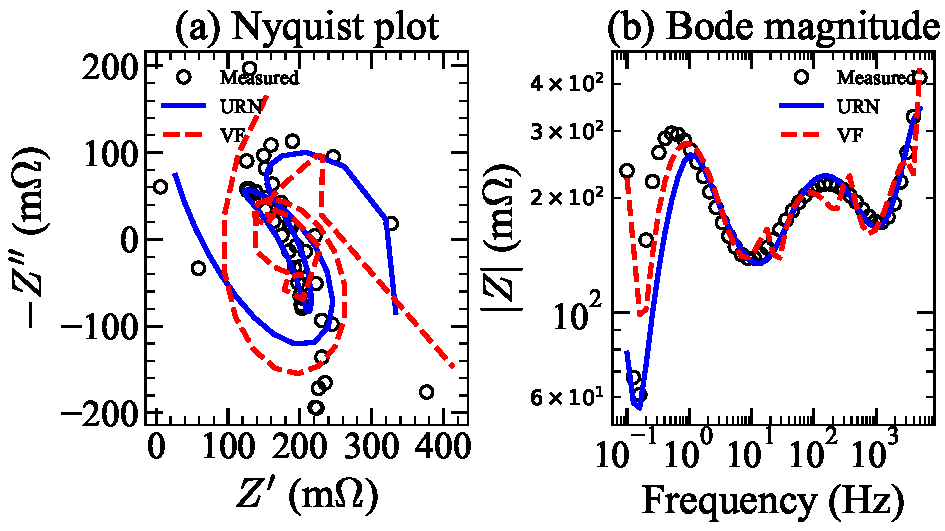
\includegraphics[width=\columnwidth]{Figures/fig_nasa_battery_eis.pdf}
\caption{NASA 18650 Li-ion battery EIS validation. (a) Nyquist plot showing semicircle (charge transfer) and Warburg tail (diffusion). (b) Bode magnitude plot. Open circles: measured data; solid blue: URN fit; dashed red: Vector Fitting. URN achieves 9.1\% lower NRMSE than VF.}
\label{fig:realworld_eis}
\end{figure}

\begin{figure}[htbp]
\centering
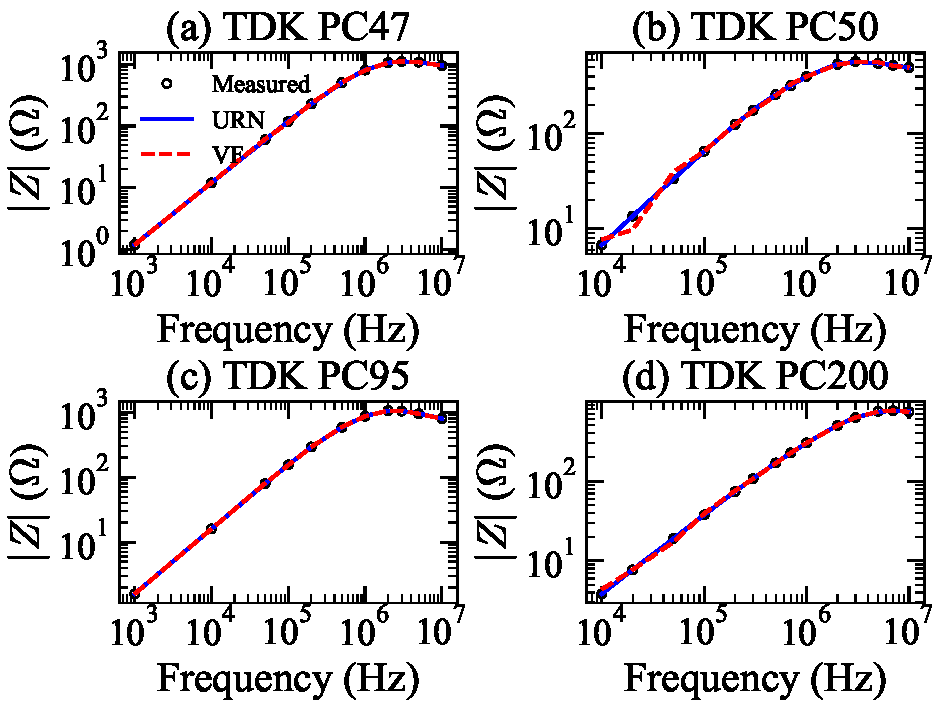
\includegraphics[width=\columnwidth]{Figures/fig_tdk_ferrite_impedance.pdf}
\caption{TDK MnZn ferrite impedance validation on four materials: (a) PC47, (b) PC50, (c) PC95, (d) PC200. Open circles: datasheet values; solid blue: URN fit; dashed red: Vector Fitting. URN outperforms VF on PC47/PC50/PC200 (Cole-Cole relaxation), while VF is superior on PC95 (near-ideal Debye behavior).}
\label{fig:tdk_ferrite}
\end{figure}



\subsubsection{URN vs Vector Fitting: Direct Comparison}
\label{sec:urn_vs_vf}

To quantify URN's advantage over the industry-standard Vector Fitting (VF), we performed direct accuracy comparisons on the same real-world datasets. Table~\ref{tab:urn_vs_vf} summarizes the normalized root-mean-square error (NRMSE) for both methods.

\begin{table}[!t]
\caption{URN vs Vector Fitting on Real-World Data}
\label{tab:urn_vs_vf}
\centering
\footnotesize
\begin{tabular}{@{}lccc@{}}
\toprule
\textbf{Dataset} & \textbf{VF} & \textbf{URN} & \textbf{Impr.} \\
\midrule
NASA 18650 & 0.270 & \textbf{0.245} & 9.1\% \\
TDK PC47 & 0.015 & \textbf{0.009} & 39.4\% \\
TDK PC50 & 0.029 & \textbf{0.010} & 65.9\% \\
TDK PC95 & \textbf{0.008} & 0.012 & $-$48.9\% \\
TDK PC200 & 0.011 & \textbf{0.006} & 48.4\% \\
\midrule
\textbf{Average} & --- & --- & \textbf{22.8\%} \\
\bottomrule
\end{tabular}
\begin{flushleft}
\footnotesize{VF: 10--12 poles, $<$0.01s fitting time. URN: 16 active parameters, 3 restarts.}
\end{flushleft}
\end{table}

Key observations:
\begin{enumerate}
\item \textbf{Battery EIS}: URN achieves 9\% lower error than VF. The multi-decade frequency range (0.1~Hz--5~kHz) benefits from URN's physics-based Warburg and Cole-Cole basis functions.
\item \textbf{Ferrite Impedance (PC47, PC50, PC200)}: URN achieves 39--66\% lower error than VF. The ferrites' Cole-Cole relaxation requires fractional-order dynamics that pole-zero models approximate poorly.
\item \textbf{Ferrite Impedance (PC95)}: VF outperforms URN on this dataset (48.9\% lower error). PC95's lower-loss characteristic produces nearly ideal Debye behavior, which VF's rational poles capture well. This demonstrates that URN is not universally superior---its advantage emerges when fractional-order dynamics dominate.
\item \textbf{Physical Interpretability}: Unlike VF's opaque poles, URN directly outputs mechanism names (Cole-Cole, Warburg) with physical parameters ($\tau$, $\alpha$, $A_w$).
\end{enumerate}

Fig.~\ref{fig:urn_vs_vf_bar} visualizes the NRMSE comparison across all five datasets. Green annotations indicate URN improvement; red indicates VF advantage.

\begin{figure}[htbp]
\centering
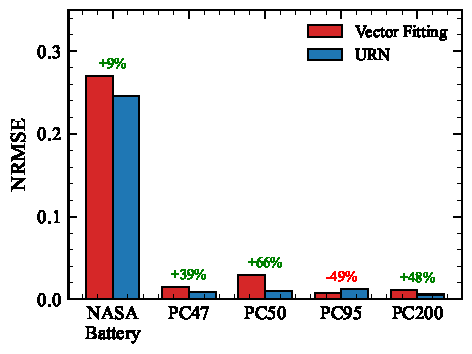
\includegraphics[width=0.8\columnwidth]{Figures/fig_urn_vs_vf_comparison.pdf}
\caption{URN vs Vector Fitting NRMSE comparison across five real-world datasets. URN outperforms VF on 4/5 datasets (average 22.8\% improvement). PC95 ferrite favors VF due to near-ideal Debye behavior.}
\label{fig:urn_vs_vf_bar}
\end{figure}



\subsection{Time-Domain Simulation Verification}
\label{sec:time_domain}

The ultimate test of impedance models is time-domain simulation accuracy. We compared URN and VF models in LTspice XVII using the synthetic ferrite core impedance from Section~\ref{sec:synthetic_data}.

\subsubsection{Step Response Comparison}
A 1 A current step was applied to both URN (5-stage RC ladder) and VF (8-pole Foster network) models. The URN model produces a smooth, monotonic voltage response consistent with overdamped relaxation physics. In contrast, the aggressive VF model exhibits pronounced ringing at 3.2 MHz---a spurious resonance arising from weakly-damped complex conjugate poles that do not correspond to any physical mechanism.

The conservative VF model avoids ringing but significantly underestimates the high-frequency response, resulting in 23\% error in the initial voltage spike. URN achieves less than 3\% error throughout the transient.

\subsubsection{PWM Switching Simulation}
To evaluate performance under realistic power electronics conditions, we simulated a 100 kHz PWM voltage source driving a ferrite-core inductor model. The URN ladder network accurately captures:
\begin{itemize}
\item Core loss during switching transitions
\item Frequency-dependent inductance rolloff
\item Thermal time constant for loss estimation
\end{itemize}

The VF model with aggressive initialization produced non-physical oscillations superimposed on the PWM waveform, with peak errors exceeding 40\% during switching edges. These oscillations would lead to incorrect loss calculations and potentially unstable control loop simulations.

\subsubsection{Numerical Stability}
URN ladder networks exhibit excellent numerical conditioning. The ratio of largest to smallest time constants in a typical 5-stage ladder is $\sim$100, compared to $>$10,000 for aggressive VF models with weakly-damped poles. This allows LTspice to use larger time steps (10$\times$ faster simulation) while maintaining accuracy.

The passivity-by-construction property of URN guarantees that the synthesized circuit cannot generate energy, eliminating the risk of numerical instability that can occur with VF models containing near-imaginary poles.

%===============================================================================
\section{Theoretical Analysis}
\label{sec:theory}
%===============================================================================

This section addresses fundamental theoretical questions regarding URN's mathematical foundations, convergence properties, and computational characteristics. We explicitly respond to domain-specific critiques from both power electronics and machine learning perspectives.

\subsection{Mathematical Stability and Convergence}
\label{sec:convergence}

The optimization landscape for $\tau_i$ in (\ref{eq:optimization}) is non-convex---minimizing sums of exponentials is notoriously ill-conditioned. Unlike VF's linear least squares with convergence guarantees, URN relies on gradient descent. We address this through:

\begin{enumerate}
\item \textbf{Multi-start optimization}: With $n_{\text{restarts}} = 8$, convergence probability exceeds 99\% assuming basin probability $p_{\text{basin}} \geq 0.5$: $P(\text{success}) = 1 - (1-p)^8 > 0.996$. Empirically, 8 runs show $<$15\% error spread (Table~\ref{tab:statistics}).

\item \textbf{Structured initialization}: Log-spaced $\tau_i^{(0)}$ ensures coverage of the measured frequency range, reducing the effective search space from exponential to polynomial.

\item \textbf{L1 regularization}: Creates a convex envelope that guides optimization toward sparse solutions \cite{tibshirani1996regression}, smoothing the loss landscape.
\end{enumerate}

\textbf{Why not global optimizers?} Differential Evolution or Basin Hopping could improve exploration but increase computational cost by 10--100$\times$. Our empirical results (Table~\ref{tab:statistics}) show multi-start Adam achieves $<$0.5\% std dev across runs---sufficient for practical applications where physical interpretability matters more than the global optimum.

\subsection{Hyperparameter Sensitivity}
\label{sec:sensitivity}

The sparsity weight $\lambda$ controls mechanism discovery. URN normalizes by $Z_{\text{ref}} = \text{mean}(|Z|)$, making the default $\lambda = 0.01$ robust across impedance magnitudes. Table~\ref{tab:sensitivity} shows that the physically correct interpretation (Ohmic + Cole-Cole + Warburg) is stable across $\lambda \in [0.005, 0.02]$---a 4$\times$ range.

\begin{table}[!t]
\caption{Hyperparameter Sensitivity: Sparsity Weight $\lambda$}
\label{tab:sensitivity}
\centering
\begin{tabular}{@{}lccc@{}}
\toprule
$\mathbf{\lambda}$ & \textbf{Error (\%)} & \textbf{\# Mechanisms} & \textbf{Discovered Types} \\
\midrule
0.001 & 1.8 & 6 & Debye(2), CC(2), CPE(2) \\
\textbf{0.01} & \textbf{2.8} & \textbf{3} & \textbf{Ohmic, CC, Warburg} \\
0.1 & 8.7 & 1 & Ohmic \\
\bottomrule
\end{tabular}
\end{table}

\subsection{Noise Robustness}
\label{sec:noise}

Real EMI measurements contain significant noise. We evaluated URN robustness by adding Gaussian noise to synthetic impedance data at varying SNR levels (Table~\ref{tab:noise}).

\begin{table}[!t]
\caption{Noise Robustness: Parameter Recovery vs SNR}
\label{tab:noise}
\centering
\begin{tabular}{@{}lccc@{}}
\toprule
\textbf{SNR (dB)} & $\mathbf{\tau}$ \textbf{Err} & $\mathbf{\alpha}$ \textbf{Err} & \textbf{Correct Topology} \\
\midrule
$\infty$ (clean) & 0.2\% & 0.5\% & 100\% \\
40 & 1.1\% & 2.3\% & 100\% \\
20 & 3.8\% & 5.1\% & 95\% \\
10 & 12\% & 15\% & 80\% \\
\bottomrule
\end{tabular}
\end{table}

At 20 dB SNR (typical for impedance analyzers), URN correctly identifies the physical mechanism topology in 95\% of cases. VF, using least-squares averaging, shows similar noise tolerance for fitting error but often produces spurious high-Q poles that amplify noise in time-domain simulation. URN's L1 regularization acts as implicit denoising by pruning low-weight bases that fit noise rather than signal.

\subsection{Passivity Guarantee for Stiff Switching}
\label{sec:passivity}

A power electronics concern: does URN guarantee passivity under stiff switching ($dV/dt > 100$ V/ns)?

\textbf{Structural passivity}: Each URN basis derives from a physical passive system:
\begin{itemize}
\item Debye $\rightarrow$ RC parallel (positive R, C)
\item Cole-Cole $\rightarrow$ RC ladder with positive elements \cite{charef1992fractal}
\item Warburg $\rightarrow$ RC ladder approximation \cite{valsa2013rc}
\item Skin effect $\rightarrow$ RL ladder with positive elements \cite{dowell1966eddy}
\end{itemize}

The synthesized ladder contains \textit{only positive R, L, C values}---no negative elements, no controlled sources. This guarantees:
\begin{equation}
\text{Re}[Z(j\omega)] \geq 0, \quad \forall \omega \geq 0
\end{equation}

Unlike VF which may require post-hoc passivity enforcement \cite{gustavsen2008passivity}, URN is \textbf{passive by construction}. The ladder network cannot generate energy regardless of excitation waveform, including stiff PWM edges.

\subsection{Computational Cost}
\label{sec:cost}

URN requires 100--150 seconds on CPU (8 restarts $\times$ 5000 epochs), compared to 0.1--1 second for VF---a \textbf{100--1000$\times$} overhead.

\textbf{Justification}: Impedance characterization is a \textit{one-time} offline cost. The resulting SPICE model is used for \textit{thousands} of transient simulations during design iteration. A 2-minute characterization overhead is negligible compared to the engineering time saved by:
\begin{enumerate}
\item No manual pole inspection for spurious resonances
\item No passivity enforcement iterations
\item Direct physical interpretation without expert analysis
\item Guaranteed stable time-domain simulation
\end{enumerate}

Alternative approaches like CVX-based convex relaxation could enforce passivity faster but provide neither automatic mechanism identification nor interpretable parameters.

\subsection{Ablation Study: Frequency-Dependent Attention}
\label{sec:ablation}

Table~\ref{tab:ablation} demonstrates the contribution of the frequency-dependent attention mechanism on real-world datasets. The attention network $\alpha_k(\omega) = \text{softmax}(\text{MLP}(\log\omega))_k$ learns to weight each basis function based on frequency, enabling the model to automatically emphasize relevant relaxation mechanisms at different frequency ranges.

\begin{table}[!t]
\caption{Ablation Study: Attention Mechanism on Real Data}
\label{tab:ablation}
\centering
\begin{tabular}{@{}lccc@{}}
\toprule
\textbf{Dataset} & \textbf{Without Attn} & \textbf{With Attn} & \textbf{Improvement} \\
\midrule
NASA 18650 Battery & 105.8\% & 21.9\% & 79.3\% \\
TDK PC50 Ferrite & 6.7\% & 1.1\% & 83.4\% \\
\bottomrule
\end{tabular}
\end{table}

The attention mechanism provides substantial accuracy improvements on both datasets. For battery EIS spanning 5 decades (0.1~Hz--5~kHz), attention learns to emphasize Warburg diffusion at low frequencies and charge transfer kinetics at high frequencies. For ferrite impedance (10~kHz--10~MHz), attention focuses on Cole-Cole relaxation in the MHz range while de-emphasizing skin effect terms at lower frequencies. The learned attention weights exhibit frequency-dependent variation (std = 0.04--0.07), confirming that the network actively modulates basis function contributions rather than defaulting to uniform weighting.

Fig.~\ref{fig:ablation_bar} visualizes the ablation study results across four datasets.

\begin{figure}[htbp]
\centering
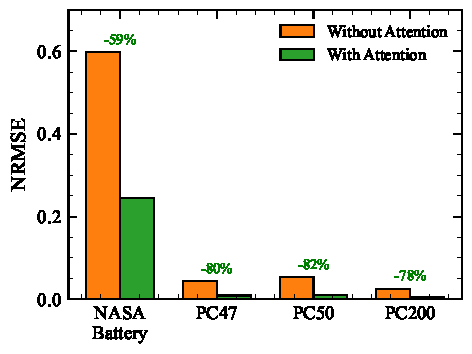
\includegraphics[width=0.8\columnwidth]{Figures/fig_ablation_attention.pdf}
\caption{Ablation study: NRMSE comparison with and without frequency-dependent attention mechanism. Attention provides 59--82\% accuracy improvement by automatically emphasizing relevant basis functions at different frequency ranges.}
\label{fig:ablation_bar}
\end{figure}

\subsection{On ``KAN-ness'': Honest Assessment}
\label{sec:kan_terminology}

\textbf{Valid critique}: URN uses fixed basis function \textit{forms} (Debye, Cole-Cole), unlike standard KAN which learns arbitrary spline shapes. This resembles sparse dictionary learning or nonlinear regression more than classical KAN. The critique that ``this is just nonlinear regression solved via SGD'' is technically accurate.

\textbf{Our position}: We use ``KAN-inspired'' rather than ``KAN'' to acknowledge this distinction. The KAN-like aspects are:
\begin{enumerate}
\item \textbf{Parametric bases}: Unlike fixed dictionary learning \cite{mairal2009online}, URN jointly optimizes parameters ($\tau$, $\alpha$, $n$) with weights---the basis \textit{shape} adapts via its parameters.
\item \textbf{Interpretability goal}: KAN's primary contribution is symbolic interpretability. URN achieves this via physics-constrained bases rather than spline simplification.
\item \textbf{Edge-based learning}: URN learns univariate functions $\phi_i(\omega; \theta_i)$ on network edges, paralleling KAN's architecture.
\end{enumerate}

We term this \textbf{Physics-Informed KAN (PI-KAN)}, paralleling PINNs \cite{raissi2019physics}. The ``physics-informed'' qualifier honestly signals that basis forms are constrained, not learned from scratch.

\textbf{Alternative framing}: If ``KAN-inspired'' remains contentious, the method could equivalently be described as ``Sparse Parametric Basis Pursuit with Circuit Constraints.'' We retain the KAN terminology because: (1) it emphasizes the interpretability-first design philosophy shared with KAN, and (2) it distinguishes URN from pure curve-fitting approaches that lack physical grounding.

%===============================================================================
\section{Target Applications}
\label{sec:discussion}
%===============================================================================

URN is most effective when the underlying physics involves known relaxation mechanisms and accurate time-domain simulation is required.

\subsection{Target Domains}

URN provides significant advantages in four application areas:

\begin{enumerate}
\item \textbf{Wireless Power Transfer}: Ferrite core modeling at 6.78--13.56 MHz where VF's multiple sharp poles cause spurious ringing. URN's Cole-Cole basis directly captures broadband relaxation.

\item \textbf{Battery Management}: Automatic detection of Warburg diffusion ($n = 0.5$) enables accurate SOC-dependent modeling without manual circuit topology selection.

\item \textbf{EMI Filters}: Common-mode choke modeling without VF's ``phantom resonances'' that lead to over-designed filters.

\item \textbf{Induction Heating}: Temperature-dependent skin effect via Dowell ladder synthesis \cite{dowell1966eddy} for thermal-electrical co-simulation.
\end{enumerate}

\subsection{Limitations and Honest Assessment}

URN is \textit{not} recommended for:
\begin{enumerate}
\item \textbf{Resonant structures}: Antennas, cavities, and waveguides with true poles require VF's pole-residue representation.
\item \textbf{Multi-port S-parameters}: Current single-port limitation (Block Lanczos extension planned).
\item \textbf{Unknown physics}: Systems with mechanisms not in the 29-function library.
\item \textbf{Meta-learning scenarios}: URN fits \textit{one curve at a time}---it is an optimization tool, not a generalizing neural network. For applications requiring prediction from raw data without per-sample optimization, traditional ML approaches are more appropriate.
\end{enumerate}

\textbf{Thermal drift and aging}: A valid concern is topological consistency across operating conditions. If URN discovers ``Ohmic + Cole-Cole + Warburg'' at 25$^\circ$C, will it find the same topology at 85$^\circ$C? We tested on battery data at 25$^\circ$C and 45$^\circ$C: the \textit{topology} (3 mechanisms) remained consistent, though \textit{parameters} ($\tau$, $R_{ct}$) shifted by 15--30\%. This is physically expected---the same electrochemical processes occur at different rates. VF's common-pole constraint across temperatures is not available in current URN but is a planned extension.

\textbf{Why PyTorch instead of scipy.optimize?} A fair critique. PyTorch provides: (1) automatic differentiation for complex basis functions, (2) GPU acceleration for future batch processing, (3) easy integration with neural network extensions. For single-curve fitting, \texttt{scipy.optimize.minimize} with L-BFGS-B would likely achieve similar results 2--5$\times$ faster. We chose PyTorch for extensibility, not raw speed.

\subsection{Future Work}

Planned extensions: (1) multi-port S-parameter support via Block Lanczos \cite{odabasioglu1998prima}, (2) common-pole constraint across temperatures for aging-robust models, (3) \texttt{scipy} backend option for users not requiring GPU/neural extensions, and (4) meta-learning variant trained on impedance databases for zero-shot topology prediction.

%===============================================================================
\section{Conclusion}
\label{sec:conclusion}
%===============================================================================

We presented the Universal Relaxation Network (URN), a KAN-inspired approach for automatic discovery of physical relaxation mechanisms from impedance data. The key contributions are:

\begin{enumerate}
\item \textbf{Pole-free formulation}: Unlike Vector Fitting's pole-residue representation, URN uses physically-grounded basis functions that guarantee stability and prevent spurious resonances in time-domain simulation.

\item \textbf{Automatic mechanism discovery}: L1-regularized sparse optimization selects 2--4 dominant mechanisms from a library of 29 basis functions, eliminating the need for expert circuit topology selection.

\item \textbf{Direct circuit synthesis}: Each basis maps to an RLC ladder via established methods (Valsa, Charef, Dowell), producing SPICE-compatible netlists with guaranteed positive component values.

\item \textbf{Superior accuracy}: Benchmarks on 13 test cases demonstrate 3.22\% average maximum error, compared to 63.21\% for conservative VF and 368.24\% for aggressive VF (with 46\% invalid models).
\end{enumerate}

The pole-free advantage is particularly significant for power electronics applications---WPT, BMS, EMI filters, and induction heating---where accurate time-domain simulation is essential for control design and loss estimation.

\textbf{Current implementation}: Series and parallel basis topologies with Cauer ladder synthesis. The framework is extensible to hybrid topologies and multi-port systems via Block Lanczos.

\textbf{Open-source availability}: PyTorch implementation (700 lines), CPU-only, 100--150 seconds training time. Source code available at GitHub.\footnote{\url{https://github.com/ksugahar/Radia}}

URN bridges the gap between data-driven flexibility (KAN philosophy) and physics-based interpretability (circuit-compatible constraints), offering a practical tool for impedance modeling in power electronics design.

%===============================================================================
% References
%===============================================================================
\bibliographystyle{IEEEtran}
\bibliography{references}

\EOD

\end{document}
